\documentclass[11pt]{article}

\usepackage[utf8]{inputenc}
\usepackage[czech]{babel}

\usepackage{libertinus}
\usepackage[T1]{fontenc}

\usepackage[a4paper, left=30mm, right=20mm, top=25mm, bottom=25mm]{geometry}

\usepackage{csquotes}
\usepackage{tabularx}
\usepackage{graphicx}


%========================================================================

\begin{document}
    \section{Uživatelská dokumentace}
    \subsection{Základní funkce}
    Obrazovka je rozdělena na dvě hlavní části - vlevo je boční panel s nástroji, respektive seznamem geometrický objektů, a vpravo je prostor pro rýsování (\textit{plátno}). Dále nahoře je záložka \textit{File}, ve které je možné narýsované objekty uložit do souboru (\textit{Save}), zpětně ze souboru načíst (\textit{Open}) nebo uložit objetky jako obrázek (\textit{Save~As}). Druhá záložka \textit{Edit} slouží k vrácení poslední změny (\textit{Undo}) a opětovného vykonání po vrácení poslední změny (\textit{Redo}). Kdykoliv zmáčknutím klávesy \textit{Delete} je možné odstranit vybrané objekty. Tažením hranice mezi bočním panelem a plátnem je možné změnit šířku bočního panelu.
    \begin{figure}[h]
        \begin{center}
        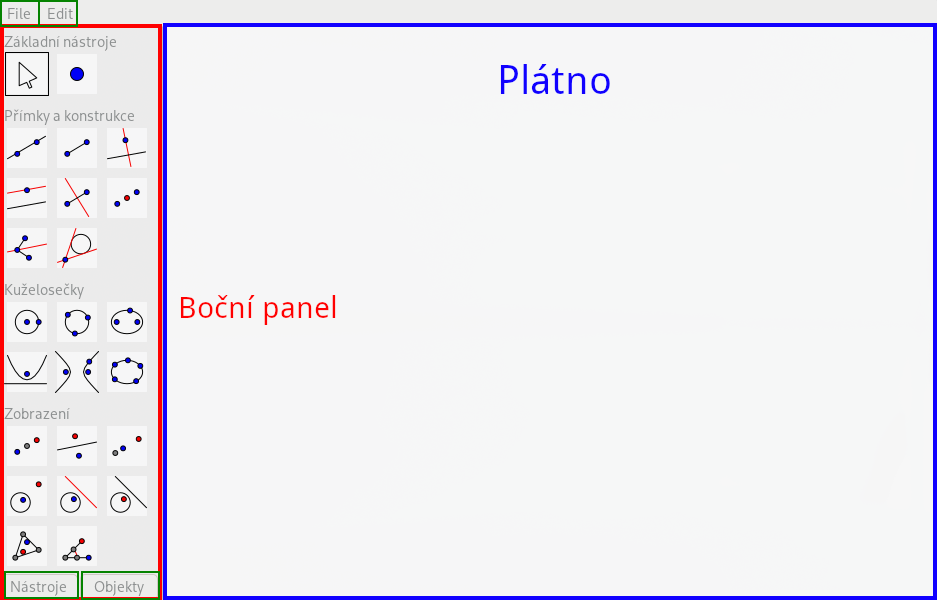
\includegraphics[scale=0.4]{imgs/overview.png}
        \end{center}
    \end{figure}
    \subsection{Nástroje}
    Na panel nástrojů je možné přepnout kliknutím na tlačítko \textit{Nástroje}, které se nachází vespod bočního panelu. Během používání libovolného nástroje je možné plátno přiblížit a oddálit pomocí kolečka myši. Zároveň kliknutím pravého tlačítka myši se nástroj \enquote{resetuje}, tedy například při chybném zvolení objektu je možné tento výběr zrušit. Dále pokud nástroj očekává výběr bodu a uživatel klikne na místo, kde se bod nenáchází, tak na daném místě vznikne bod podle \ref{point}.

    \subsubsection{Základní nástroje}
    \vspace{-10pt}
    \begin{figure}[h]
        \begin{center}
        
\includegraphics[scale=0.5]{imgs/basic_tools.png}
        \end{center}
    \end{figure}
    \vspace{-25pt}
    \begin{enumerate}
        \item{\bf Ukazovátko} \\
        Tímto nástrojem je možné hýbat body, která jsou volné nebo přichycené k nějaké křivce. Také je možné hýbat celým plátnem potažením libovolného prázdného místa.
        \item{\bf Bod} \label{point}\\
        Tímto nástrojem je možné vytvářet body. Kliknutím na místo, kde se nenáchází žádná křivka vznikne volně pohyblivý bod. Kliknutím na místo, kde se nachází jedna křivka, vznikne bod, který je k této křivce \enquote{přichycený}, tedy je možné s tímto bodem stále hýbat ale pouze po této křivce. Kliknutím na místo, kde se nachází více křivek, vznikne bod, který leží na průsečíku dvou nejbližších křivek.
    \end{enumerate}

    \subsubsection{Přímky a konstrukce}
    \vspace{-10pt}
    \begin{figure}[h]
        \begin{center}
        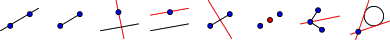
\includegraphics[scale=0.5]{imgs/line_tools.png}
        \end{center}
    \end{figure}
    \vspace{-25pt}
    \begin{enumerate}
        \item{\bf Přímka dvěma body}\\
        Tento nástroj vytvoří přímku procházející dvěma různými body. Tyto body se postupně označit kliknutím.
        \item{\bf Úsečka}\\
        Tento nástroj vytvoří úsečku s dvěma různými koncovými body. Tyto body se postupně označit kliknutím.
        \item{\bf Kolmice}\\
        Tento nástroj vytvoří přímku kolmou ke křivce procházející daným bodem. Danou křivku a bod stačí označit kliknutím v libovolném pořadí. (Průsečíkem s křivkou je možné získat nejbližší bod na křivce.)
        \item{\bf Rovnoběžka}\\
        Tento nástroj vytvoří přímku rovnoběžnou ke křivce procházející daným bodem. Danou křivku a bod stačí označit kliknutím v libovolném pořadí.
        \item{\bf Osa úsečky}\\
        Tento nástroj vytvoří přímku, která je osou dané úsečky. Kliknutím se označí krajní body dané úsečky.
        \item{\bf Střed}\\
        Tento nástroj vytvoří střed úsečky, případně kuželosečky. Při kliknutí na úsečku nebo kuželosečku se střed rovnou vytvoří. Je možné také klinkout na dva body, čímž vznikne střed úsečky tvořené těmito body.
        \item{\bf Osa úhlu}\\
        Tento nástroj vytvoří osu úhlu. Je možné buď zvolit tři body, kde prostřední je vrchol daného úhlu a zbylé dva leží na jeho ramenech, nebo dvě přímky/úsečky, které tvoří ramena úhlu.
        \item{\bf Tečna}\\
        Tento nástroj vytvoří tečny z daného bodu ke kuželosečce. Bod a kuželosečku je možné vybrat v libovolném pořadí. Pro konstrukci body dotyku je možné využít nástroj \textit{Pól}.
    \end{enumerate}

    \subsubsection{Kuželosečky}
    \vspace{-10pt}
    \begin{figure}[h]
        \begin{center}
        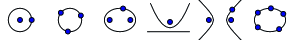
\includegraphics[scale=0.5]{imgs/conic_tools.png}
        \end{center}
    \end{figure}
    \vspace{-25pt}
    \begin{enumerate}
        \item{\bf Kružnice se středem}\\
        Tento nástroj vytvoří kružnici s daným středem a bodem, který na kružnici leží. Jako první je třeba vybrat střed a bod na kužnici jako druhý.
        \item{\bf Kružnice třemi body}\\
        Tento nástroj vytvoří kružnici procházející třemi danými body. Tyto body je možné vybrat v libovolném pořadí.
        \item{\bf Elipsa}\\
        Tento nástroj vytvoří elipsu danou dvěma ohnisky a bodem ležící na ní. Jako první je třeba vybrat obě ohniska a až poté bod na elipse.
        \item{\bf Parabola}\\
        Tento nástroj vytvoří parabolu danou ohniskem a řídící přímkou. Přímku a bod je možné vybrat v libovolném pořadí.
        \item{\bf Hyperbola}\\
        Tento nástroj vytvoří hyperbolu danou dvěma ohnisky a bodem ležící na ní. Jako první je třeba vybrat obě ohniska a až poté bod na hyperbole.
        \item{\bf Kuželosečka pěti body}\\
        Tento nástroj vytvoří kuželosečku vedenou pěti body. Tyto body je možné zvolit v libovolném pořadí.
    \end{enumerate}

    \subsubsection{Zobrazení}
    \vspace{-10pt}
    \begin{figure}[h]
        \begin{center}
        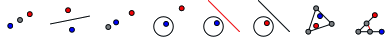
\includegraphics[scale=0.5]{imgs/transform_tools.png}
        \end{center}
    \end{figure}
    \vspace{-25pt}
    \begin{enumerate}
        \item{\bf Středová souměrnost}\\
        Tento nástroj zobrazí objekt ve středové souměrnosti. Jako první je třeba zvolit vzor a až poté střed souměrnosti.
        \item{\bf Osová souměrnost}\\
        Tento nástroj zobrazí objekt v osové souměrnosti. Jako první je třeba zvolit vzor a až poté osu souměrnosti.
        \item{\bf Stejnolehlost}\\
        Tento nástroj zobrazí objekt ve stejnolehlosti s daným středem a koeficientem. Jako první je potřeba zvolit vzor a až poté střed stejnolehlosti. Pak je potřeba zadat koeficient stejnolehlosti.
        \item{\bf Kruhová inverze}\\
        Tento nástroj zobrazí bod v kruhové inverzi podle dané kružnice. Daný bod a kružnici je možné zvolit v libovolném pořadí. (Není možné zobrazit střed dané kružnice.)
        \item{\bf Polára}\\
        Tento nástroj vytvoří k danému bodu poláru podle dané kuželosečky. Daný bod a kuželosečku je možné zvolit v libovolném pořadí.
        \item{\bf Pól}\\
        Tento nástroj vytvoří k dané přímce pól podle dané kuželosečky. Danou přímku a kuželosečku je možné zvolit v libovolném pořadí.
        \item{\bf Kamarád (Isogonal conjugate)}\\
        Tento nástroj vytvoří k daném bodu kamaráda vzhledem k danému trojúhelníku. Jako první je třeba zvolit vrcholy referenčního trojúhelníku a poté až daný bod.
        \item{\bf Otočení}\\
        Tento nástroj otočí daný objekt o úhel. Jako první je třeba označit tři body. První z nich leží na prvním rameni úhlu, druhý je vrcholem úhlu a třetí je na výsledném rameni úhlu. Jako poslední se zvolí objekt k otočení.
    \end{enumerate}

    \subsection{Seznam objektů}
    Na seznam objektů je možné přepnout kliknutím na tlačítko \textit{Objekty} vespod bočního panelu. Jendím kliknutím na objekt v seznamu je možné daný objekt označit (držením klávesy \textit{Control} nebo \textit{Shift} je možné označit více objektů naráz). Dvojitým kliknutím na objekt je možné ho upavit. U objektu je možné upravit jeho název, definici, parametr, tloušťku hranice, barvu hranice a barvu výplně (barva výplně se vztahuje jen k bodům). Tažením hranic sloupců je možné změnit jejich šířku.
    \begin{figure}[h]
        \begin{center}
        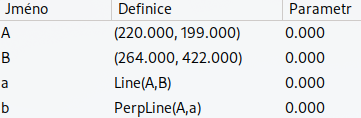
\includegraphics[scale=0.5]{imgs/obj_list.png}
        \end{center}
    \end{figure}
    \vspace{-20pt}
    \subsubsection{Parametr}
    Parametr může znamenat více věcí. U bodů přichycených ke křivce je tento parametr dán parametrizací dané křivky (tedy každý bod na křivce má svůj nějaký parametr). Dále u bodů na průsečíku křivek značí paramter index průsečíku, ke kterému je bod přichycen. U tečen parametr značí index dané tečny a u stejnolehlosti její koeficient. Na zbylé objekty nemá paramter vliv.
    \subsubsection{Definice}
    Definice objektu se skládá ze dvou částí - názvu a argumentů. Nejprve je název a poté jsou v závorkách argumenty oddělené čárkami. Všechny argumenty jsou názvy nějakých jiných objektů (záleží na velikosti písmen i mezerách), kromě volných bodů, které nemají název a místo argumentů mají dvě čísla - souřadnici x a y.
    \begin{table}[!htb]
    \begin{center}
        \caption{\bf Body}
        \begin{tabularx}{\linewidth}{|l|X|}
            \hline 
            \multicolumn{1}{|c|}{\textbf{Název + argumenty}} & \multicolumn{1}{c|}{\textbf{Vysvětlení}}\\
            \hline

            (<x>,<y>) & Volný bod se souřadnicemi <x> a <y>. \\
            \hline
            OnCurve(<Křivka>) & Bod přichycený ke křivce <Křivka>. \\
            \hline
            OnIntersect(<Křivka1>,<Křivka2>) & Bod na průsečíku <Křivka1> a <Křivka2>. \\
            \hline
            Midpoint(<Bod1>,<Bod2>) & Střed úsečky s koncovými body <Bod1> a <Bod2>. \\
            \hline
            Midpoint(<Kuželosečka>) & Střed kuželosečky <Kuželosečka>. \\
            \hline
            Midpoint(<Úsečka>) & Střed úsečky <Úsečka>. \\
            \hline
        \end{tabularx}
    \end{center}
    \end{table}

    \begin{table}[!htb]
    \begin{center}
        \caption{\bf Přímky}
        \begin{tabularx}{\linewidth}{|l|X|}
            \hline 
            \multicolumn{1}{|c|}{\textbf{Název + argumenty}} & \multicolumn{1}{c|}{\textbf{Vysvětlení}}\\
            \hline

            Segment(<Bod1>,<Bod2>) & Úsečka s koncovými body <Bod1> a <Bod2>. \\
            \hline
            Line(<Bod1>,<Bod2>) & Přímka procházející body <Bod1> a <Bod2>. \\
            \hline
            PerpLine(<Bod>,<Křivka>) & Kolmice na <Křivka> procházející <Bod>. \\
            \hline
            ParalLine(<Bod>,<Křivka>) & Rovnoběžka s <Křivka> procházející <Bod>. \\
            \hline
            PerpBisector(<Bod1>,<Bod2>) & Osa úsečky s koncovými body <Bod1> a <Bod2>. \\
            \hline
            AngleBisector(<Bod1>,<Bod2>,<Bod3>) & Osa úhlu s vrcholem <Bod2> a rameny s body <Bod1> a <Bod2>. \\
            \hline
            AngleBisector(<Přímka1>,<Přímka2>) & Osa úhlu s rameny <Přímka1> a <Přímka2>. \\
            \hline
            AngleBisectorP(<Bod1>,<Bod2>,<Bod3>) & Kolmice na osu úhlu s vrcholem <Bod2> a rameny s body <Bod1> a <Bod2>. \\
            \hline
            AngleBisectorP(<Přímka1>,<Přímka2>) & Kolmice na osu úhlu s rameny <Přímka1> a <Přímka2>. \\
            \hline
            Tangent(<Bod>,<Kuželosečka>) & Tečna skrz <Bod> ke kuželosečce <Kuželosečka>. \\
            \hline
        \end{tabularx}
    \end{center}
    \end{table}

    \begin{table}[!htb]
    \begin{center}
        \caption{\bf Kuželosečky}
        \begin{tabularx}{\linewidth}{|l|X|}
            \hline 
            \multicolumn{1}{|c|}{\textbf{Název + argumenty}} & \multicolumn{1}{c|}{\textbf{Vysvětlení}}\\
            \hline

            Conic(<Bod1>,<Bod2>,<Bod3>,<Bod4>,<Bod5>) & Kuželosečka skrz všech 5 bodů. \\
            \hline
            CircleBy2P(<Bod1>,<Bod2>) & Kružnice se středem <Bod1> procházející <Bod2>. \\
            \hline
            CircleBy3P(<Bod1>,<Bod2>,<Bod3>) & Kružnice skrz <Bod1>, <Bod2> a <Bod3>. \\
            \hline
            Ellipse(<Bod1>,<Bod2>,<Bod3>) & Elipsa s ohnisky <Bod1> a <Bod2> procházející <Bod3>. \\
            \hline
            Hyperbola(<Bod1>,<Bod2>,<Bod3>) & Hyperbola s ohnisky <Bod1> a <Bod2> procházející <Bod3>. \\
            \hline
            Parabola(<Bod>,<Přímka>) & Parabola s ohniskem <Bod> a řídící přímkou <Přímka>. \\
            \hline
        \end{tabularx}
    \end{center}
    \end{table}

    \begin{table}[!htb]
    \begin{center}
        \caption{\bf Zobrazení}
        \begin{tabularx}{\linewidth}{|l|X|}
            \hline 
            \multicolumn{1}{|c|}{\textbf{Název + argumenty}} & \multicolumn{1}{c|}{\textbf{Vysvětlení}}\\
            \hline 
            
            Pole(<Přímka>,<Kuželosečka>) & Pól přímky <Přímka> vůči kuželosečce <Kuželosečka>. \\
            \hline
            Polar(<Bod>,<Kuželosečka>) & Polára bodu <Bod> vůči kzželosečce <Kuželosečka>. \\
            \hline
            PtReflect(<Objekt>,<Bod>) & <Objekt> zobrazený ve středové souměrnosti podle <Bod>. \\
            \hline
            LineReflect(<Objekt>,<Přímka>) & <Objekt> zobrazený v osové souměrnosti podle <Přímka>. \\
            \hline
            IsoConjugate(<Bod1>,<Bod2>,<Bod3>,<Bod4>) & Kamarád bodu <Bod1> v trojúhelníku s vrcholy <Bod1>,<Bod2>,<Bod3>. \\
            \hline
            Homothety(<Objekt>,<Bod>) & <Objekt> zobrazený ve stejnolehlosti se středem <Bod>. \\
            \hline
            CircleInverse(<Bod>,<Kružnice>) & <Bod> zobrazený v kruhové inverzi podle <Kružnice>. \\
            \hline
            Rotation(<Objekt>,<Bod1>,<Bod2>,<Bod3>) & <Objekt> otočený o úhel se středem v <Bod2>, vzorovém rameni <Bod1> a obrazovém <Bod3>. \\
            \hline
        \end{tabularx}
    \end{center}
    \end{table}

    \begin{samepage}
        \subsection{Soubory}
        Plátno uložené do souboru je jednoduchý \textit{.csv} soubor oddělený středníky. Tento soubor je možné upravovat i ručně. Je v něm 6 sloupců: jméno objektu, definice, parametr, barva hranice, barva výplně a tloušťka hranice. (Barvy jsou uložené jako 32bitové číslo v dekadickém zápisu.) Pokud se program pokusí načíst soubor, který není validní, tak soubor nenačte a nic se na plátně nezmění.
        
    \end{samepage}
\end{document}